\chapter{Réalisation du Sprint 2 : Gestion des classes et visio-conférence}

\section*{Introduction}
\addcontentsline{toc}{section}{Introduction}

Le deuxième sprint du projet a été consacré à la mise en place des fonctionnalités de gestion des classes, de la planification et de la communication synchrone. Ces fonctionnalités sont essentielles pour permettre aux utilisateurs de structurer l'organisation pédagogique, de collaborer en direct via visioconférence et de superviser le déroulement des enseignements.

Ce chapitre présente les étapes du développement de ce sprint : le backlog, l'analyse fonctionnelle, la conception, la réalisation des interfaces et les tests associés.

\section{Backlog du Sprint 2}

Le backlog du Sprint 2 compile onze User Stories couvrant la gestion des classes et des plannings, ainsi que la création, le suivi, la modération et l’enregistrement des appels vidéo. Ces US ont été priorisées « Haute », « Moyenne » ou « Basse » selon leur criticité pour la continuité pédagogique. Le tableau \ref{tab:sprint2_backlog} détaille chaque US avec ses critères d’acceptation.

\begin{xltabular}{\textwidth}{|c|>{\raggedright\arraybackslash}p{4cm}|X|c|}
\hline
\textbf{ID} & \textbf{Titre} & \textbf{Critères d’acceptation} & \textbf{Priorité} \\
\hline
\endfirsthead

\multicolumn{4}{c}{{\bfseries \tablename\ \thetable{} -- suite de la page précédente}} \\
\hline
\textbf{ID} & \textbf{Titre} & \textbf{Critères d’acceptation} & \textbf{Priorité} \\
\hline
\endhead

\hline
\multicolumn{4}{|r|}{\textit{Suite sur page suivante}} \\
\endfoot

\hline
\caption{User Stories du Sprint 2 – Gestion des classes et visioconférence} \label{tab:sprint2_backlog}
\endlastfoot

US-06 & Création et gestion des classes & L’administrateur peut créer, modifier, supprimer des classes et y assigner des étudiants et un enseignant. & Haute \\
\hline
US-07 & Planification des cours & L’administrateur définit les horaires des classes (date, heure, durée) dans un emploi du temps interactif. & Haute \\
\hline
US-08 & Supervision générale & L’administrateur dispose d'une vue d'ensemble sur les utilisateurs, les classes et les activités récentes. & Moyenne \\
\hline
US-09 & Création d’un appel vidéo & L’enseignant peut démarrer une session Daily.co directement depuis le planning. & Haute \\
\hline
US-10 & Rejoindre un appel vidéo & L’étudiant rejoint la session vidéo prévue en un clic depuis son tableau de bord. & Haute \\
\hline
US-11 & Partage d’écran & L’enseignant peut partager son écran (présentation, code) avec l'ensemble des participants. & Haute \\
\hline
US-12 & Modération audio/vidéo & L’enseignant peut couper le micro ou la caméra d’un étudiant pour maintenir le calme. & Moyenne \\
\hline
US-13 & Chat de session & Les participants peuvent échanger des messages textuels en temps réel pendant l'appel vidéo. & Moyenne \\
\hline
US-14 & Détection de présence & Le système enregistre automatiquement l'heure d'arrivée, les retards et les absences des étudiants. & Haute \\
\hline
US-15 & Historique de participation & L’enseignant et l'admin peuvent consulter l’historique des présences détaillé par séance. & Haute \\
\hline
US-16 & Enregistrement et replay & Les sessions peuvent être enregistrées et consultées ultérieurement par les étudiants. & Basse \\
\hline
\end{xltabular}

\section{Analyse}

\subsection{Diagramme de cas d’utilisation du Sprint 2}
Le diagramme de cas d’utilisation (figure \ref{fig:usecase_sprint2}) illustre les interactions entre l’administrateur, l’enseignant et l’étudiant pour la gestion des classes, la planification, les notifications, les appels vidéo avec modération, chat intégré et replay.

\begin{figure}[H]
    \centering
    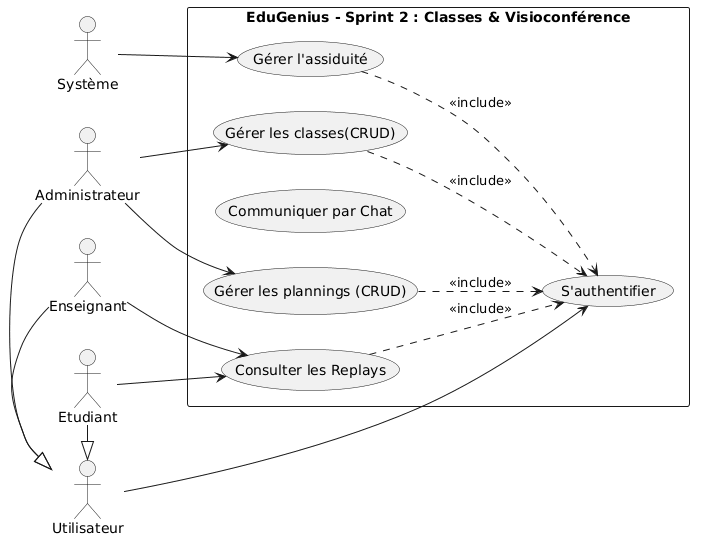
\includegraphics[width=1\textwidth]{images/use_case_diagram_sprint_2.png}
    \caption{Diagramme de cas d’utilisation – Gestion des
classes et visioconférence}
    \label{fig:usecase_sprint2}
\end{figure}

\subsection{Description textuelle des cas d’utilisation}
Cette section détaille de manière structurée les scénarios nominaux et alternatifs pour chaque cas d’utilisation clé du second sprint. Les descriptions suivent un format standardisé pour garantir une compréhension claire des interactions système et des règles métier associées.

\subsection{Cas d'utilisation : Créer une classe}
Ce cas permet à l'administrateur de créer un nouveau groupe pédagogique en définissant ses caractéristiques et son rattachement.

\begin{table}[H]
\centering
\small
\begin{tabularx}{\textwidth}{|l|X|}
\hline
\rowcolor[HTML]{EFEFEF} 
\textbf{Acteur(s)} & Administrateur \\ \hline
\textbf{Pré-conditions} & L'admin doit être authentifié et les départements doivent être configurés. \\ \hline
\textbf{Post-conditions} & La classe est créée et prête à recevoir un emploi du temps. \\ \hline
\textbf{Scénario nominal} & 
1. L'admin accède au module de création de classes. \newline
2. Il saisit les informations (Nom, Code, Année, Niveau). \newline
3. Il sélectionne le département de rattachement. \newline
4. Le système valide et persiste les données. \newline
5. La classe apparaît dans la liste des classes. \\ \hline
\textbf{Scénario alternatif} & 
2.a. Code classe existant : le système affiche une erreur de duplication. \\ \hline
\end{tabularx}
\caption{Description textuelle - Créer une classe}
\end{table}

\subsection{Cas d'utilisation : Créer un emploi du temps}
Ce cas permet à l'administrateur de définir les créneaux horaires des enseignements pour une classe donnée.

\begin{table}[H]
\centering
\small
\begin{tabularx}{\textwidth}{|l|X|}
\hline
\rowcolor[HTML]{EFEFEF} 
\textbf{Acteur(s)} & Administrateur \\ \hline
\textbf{Pré-conditions} & La classe, les matières et les enseignants doivent exister. \\ \hline
\textbf{Post-conditions} & L'emploi du temps est créé et visible par les acteurs concernés. \\ \hline
\textbf{Scénario nominal} & 
1. L'admin sélectionne une classe cible. \newline
2. Il ajoute une séance (Jour, Heure, Matière, Enseignant). \newline
3. Le système vérifie la disponibilité de l'enseignant. \newline
4. L'admin valide le planning hebdomadaire. \newline
5. L'emploi du temps est publié. \\ \hline
\textbf{Scénario alternatif} & 
3.a. Conflit d'horaire : le système signale que l'enseignant est déjà occupé sur ce créneau. \\ \hline
\end{tabularx}
\caption{Description textuelle - Créer un emploi du temps}
\end{table}

\subsection{Cas d'utilisation : Gérer l'assiduité}
Le système assure de manière autonome le suivi de la présence des étudiants lors des sessions de visioconférence.

\begin{table}[H]
\centering
\small
\begin{tabularx}{\textwidth}{|l|X|}
\hline
\rowcolor[HTML]{EFEFEF} 
\textbf{Acteur(s)} & Système \\ \hline
\textbf{Pré-conditions} & Une séance virtuelle doit être en cours. \\ \hline
\textbf{Post-conditions} & Les journaux de présence sont mis à jour en base de données. \\ \hline
\textbf{Scénario nominal} & 
1. Le système détecte l'entrée d'un étudiant dans la salle virtuelle. \newline
2. Il enregistre l'horodatage exact de connexion. \newline
3. Il surveille la durée totale de participation. \newline
4. Il génère le statut (Présent/Retard/Absent) à la fin de la séance. \\ \hline
\textbf{Scénario alternatif} & 
1.a. Déconnexion/Reconnexion : le système cumule les temps de présence fragmentés. \\ \hline
\end{tabularx}
\caption{Description textuelle - Gérer l'assiduité}
\end{table}

\subsection{Cas d'utilisation : Consulter les Replays}
Les utilisateurs accèdent aux archives vidéo des séances passées pour révision ou rattrapage.

\begin{table}[H]
\centering
\small
\begin{tabularx}{\textwidth}{|l|X|}
\hline
\rowcolor[HTML]{EFEFEF} 
\textbf{Acteur(s)} & Enseignant, Étudiant \\ \hline
\textbf{Pré-conditions} & La séance doit avoir été enregistrée et le flux traité. \\ \hline
\textbf{Post-conditions} & La vidéo est visionnée dans le lecteur intégré. \\ \hline
\textbf{Scénario nominal} & 
1. L'utilisateur accède à la médiathèque de sa classe. \newline
2. Il sélectionne une séance archivée. \newline
3. Le système récupère le flux depuis le stockage Cloud. \newline
4. Le lecteur multimédia démarre la lecture. \\ \hline
\textbf{Scénario alternatif} & 
3.a. Fichier non disponible : le système indique que le replay est en cours de traitement. \\ \hline
\end{tabularx}
\caption{Description textuelle - Consulter les Replays}
\end{table}

\section{Conception}

\subsection{Diagramme de séquence du cas : Créer une classe}
Le diagramme de séquence de la figure \ref{fig:create_class_sequence} détaille le processus administratif de structuration d'un groupe pédagogique. Ce flux illustre la coordination entre l'interface de gestion, le service d'API et la persistance en base de données. L'administrateur définit les paramètres de la classe (nom, département, niveau) et le système assure l'intégrité référentielle en liant ces entités dans la collection MongoDB, garantissant ainsi un socle solide pour la planification ultérieure des cours.

\begin{figure}[H]
    \centering
    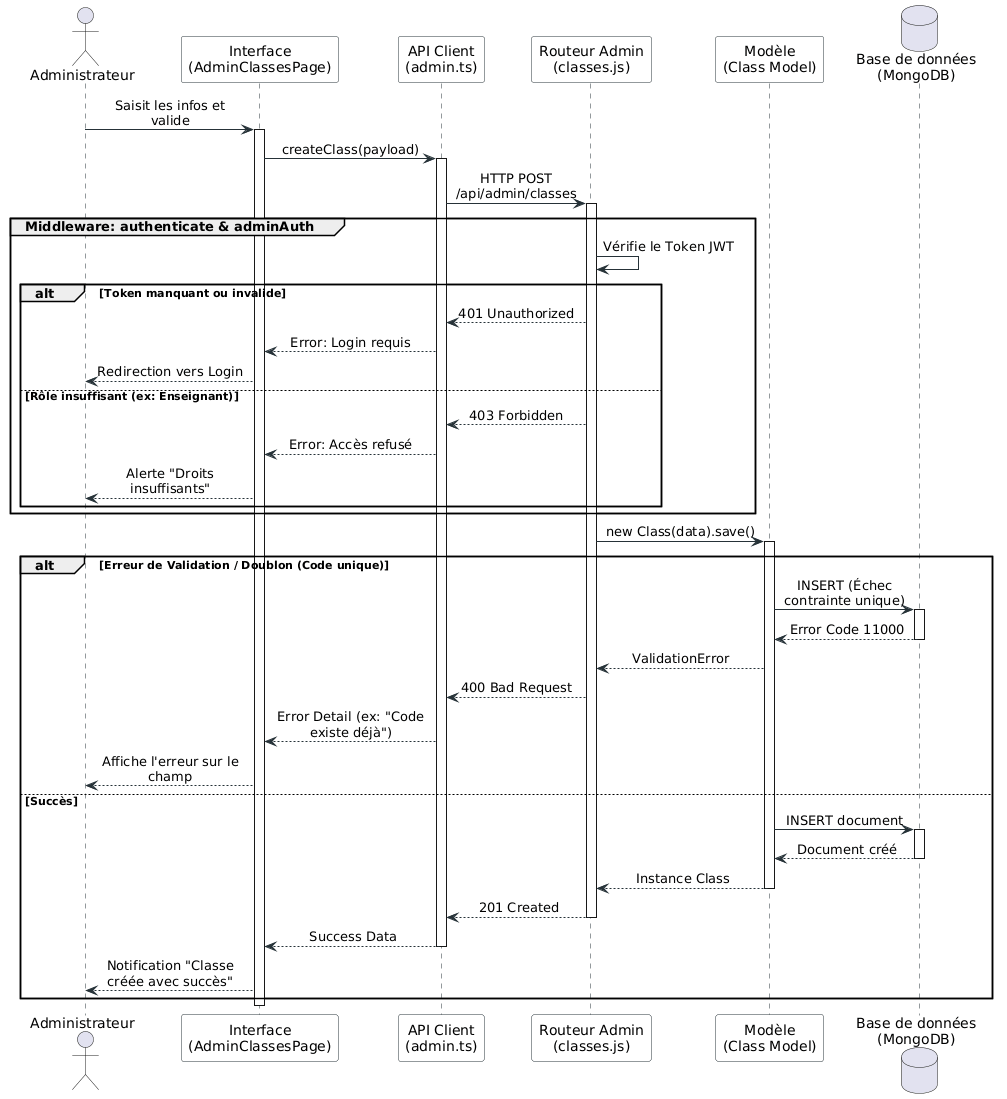
\includegraphics[width=\textwidth]{images/class_management_sequence_diagram.png}
    \caption{Diagramme de séquence – Création et configuration d'une classe (Admin)}
    \label{fig:create_class_sequence}
\end{figure}

\subsection{Diagramme de séquence du cas : Rejoindre une séance et détection de présence}
La figure \ref{fig:presence_sequence} expose le mécanisme complexe de communication synchrone et de suivi automatisé. Lorsqu'un utilisateur rejoint une salle virtuelle, le frontend initialise le SDK \textbf{Daily.co} pour établir le flux WebRTC. Simultanément, un événement de connexion déclenche un appel asynchrone vers le backend. Le système identifie l'utilisateur via son token JWT et enregistre automatiquement son horodatage d'entrée. Ce processus transparent garantit la fiabilité des relevés d'assiduité sans intervention manuelle de l'enseignant.

\begin{figure}[H]
    \centering
    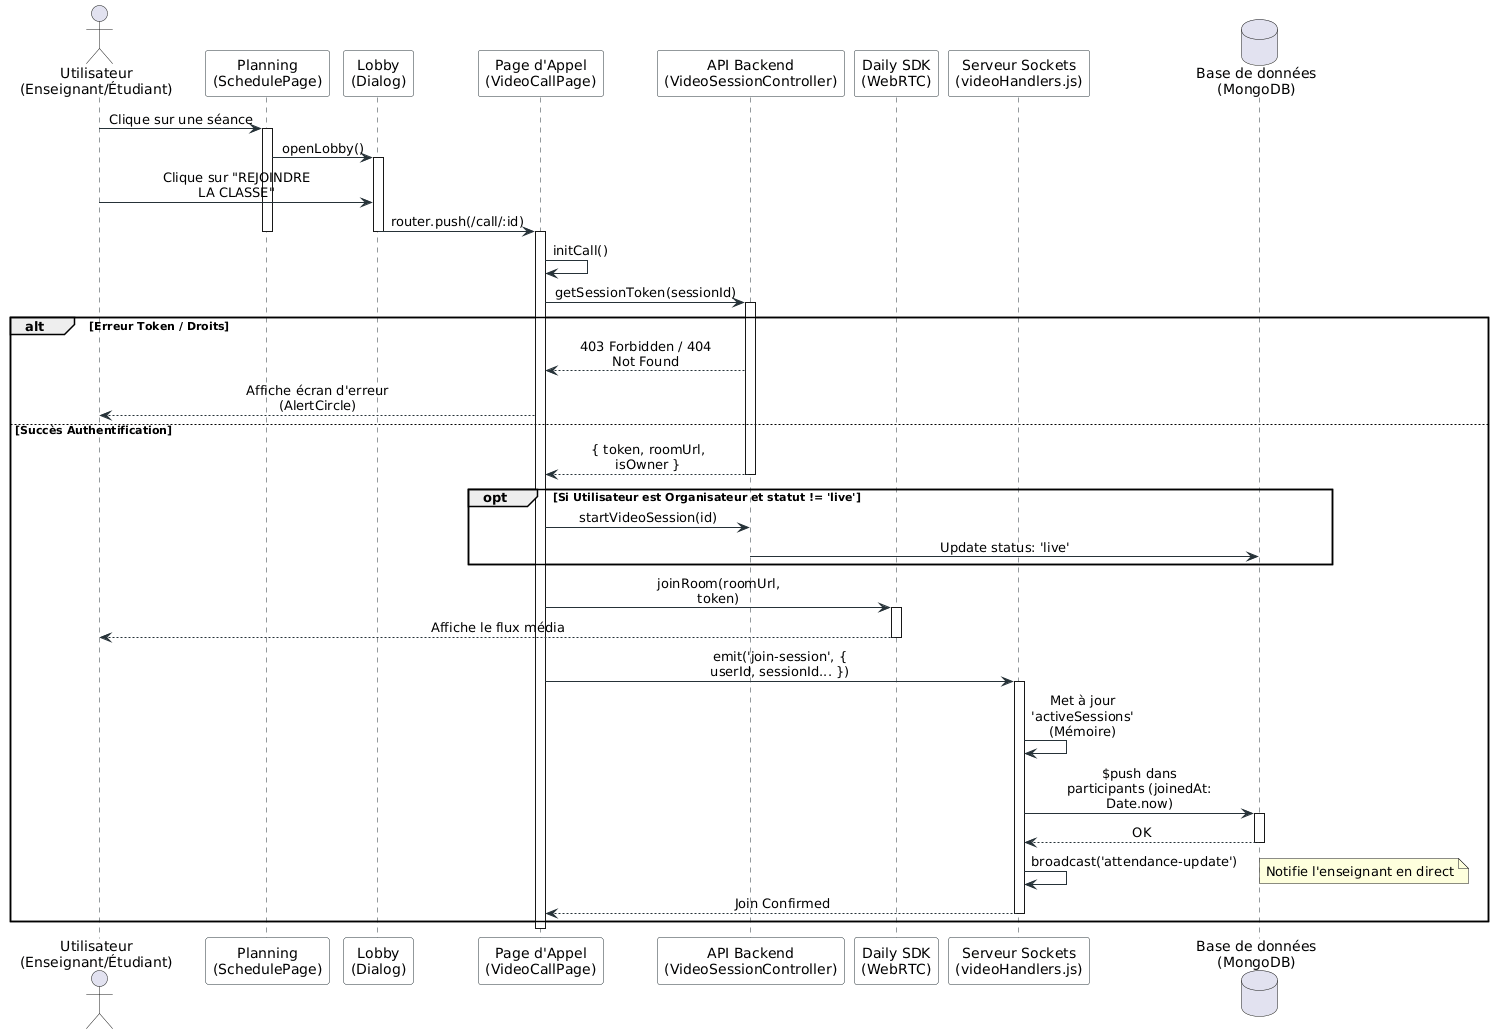
\includegraphics[width=\textwidth]{images/join_call_sequence_diagram.png}
    \caption{Diagramme de séquence – Accès à la visioconférence et suivi de présence automatique}
    \label{fig:presence_sequence}
\end{figure}

\subsection{Diagramme de classes du Sprint 2}
La figure \ref{fig:class_sprint2} présente le modèle structurel du second sprint, centré sur la gestion des classes et la communication synchrone. L'entité centrale \texttt{Class} s'enrichit de méthodes de gestion des effectifs (\texttt{joinClass}, \texttt{assignTeacher}). La planification est assurée par le modèle \texttt{Schedule} et ses entrées détaillées (\texttt{ScheduleEntry}). Le cœur de la visioconférence repose sur \texttt{VideoSession}, qui orchestre les interactions avec l'API Daily.co et génère, à sa clôture, une entité \texttt{Attendance}. Ce diagramme met également en évidence l'intégration des profils \texttt{Teacher} et \texttt{Student} au sein de l'objet \texttt{User}, assurant une spécialisation des données sans complexifier l'héritage en base.

\begin{figure}[H]
    \centering
    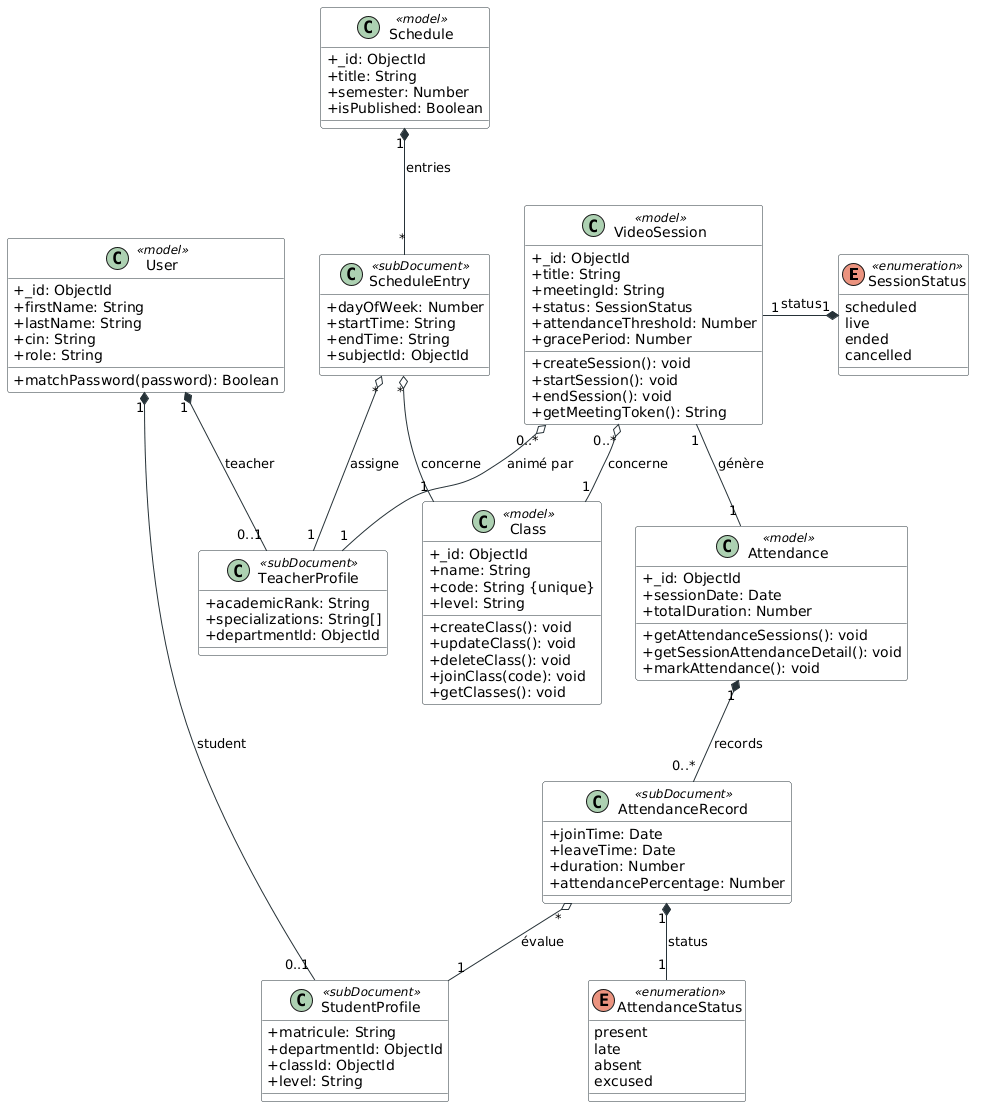
\includegraphics[width=\textwidth]{images/class_diagram_sprint_2.png}
    \caption{Diagramme de classes – Gestion des classes, sessions vidéo et suivi d'assiduité}
    \label{fig:class_sprint2}
\end{figure}

\subsection{Représentation graphique de la base de données}
Le schéma physique de la base de données (figure \ref{fig:mongodb_sprint2}) illustre la transition d'EduGenius vers un système de gestion pédagogique complet. L'architecture NoSQL a été optimisée pour supporter des requêtes complexes sur les emplois du temps et les statistiques de présence.

La collection \texttt{classes} agit comme le pivot organisationnel, liant les départements aux utilisateurs. Elle stocke de manière atomique les tableaux d'enseignants et d'étudiants, facilitant ainsi les contrôles d'accès lors des sessions live. La gestion temporelle est déléguée à la collection \texttt{schedules}, dont la structure par entrées permet de définir des cycles hebdomadaires récurrents.

Le suivi de la communication synchrone repose sur un couplage fort entre \texttt{videosessions} et \texttt{attendances}. Tandis que la première conserve les métadonnées techniques de l'appel (URLs, jetons Daily.co, paramètres de modération), la seconde centralise les rapports d'assiduité calculés. Cette séparation permet de purger les logs techniques de session tout en conservant l'historique pédagogique des présences, optimisant ainsi l'espace de stockage sur le long terme.

\begin{figure}[H]
    \centering
    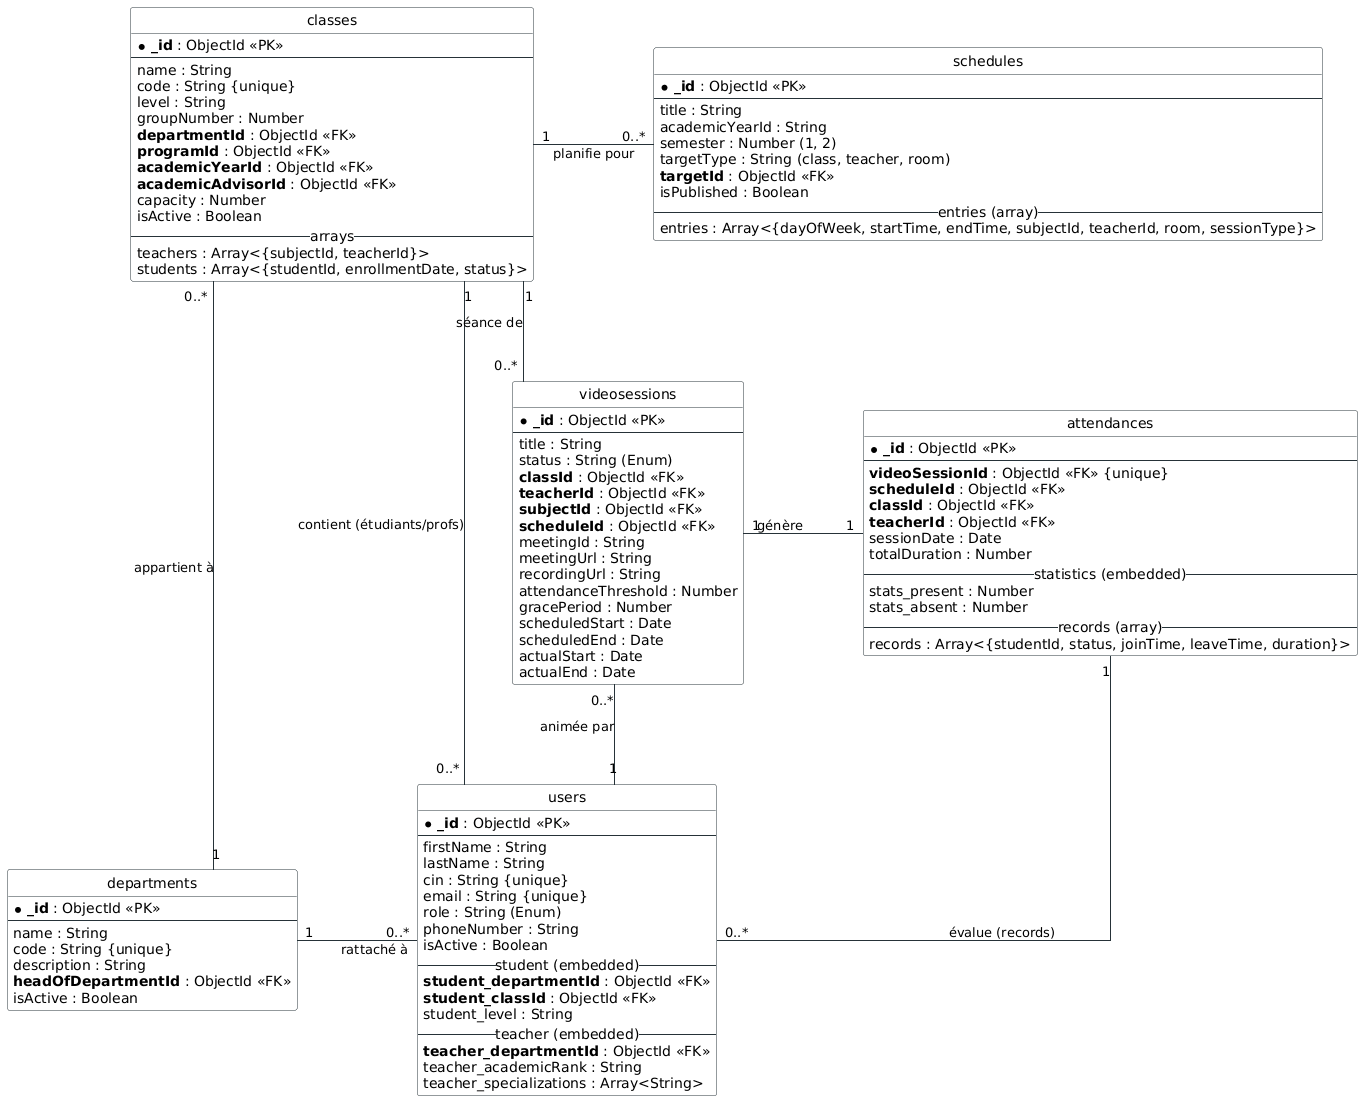
\includegraphics[width=\textwidth]{images/ERD_sprint_2.png}
    \caption{Schéma des collections MongoDB pour le sprint 2}
    \label{fig:mongodb_sprint2}
\end{figure}

\section{Réalisation}

\subsection{Interface de gestion des classes (Admin)}

L'interface de gestion des classes présente une vue en cartes avec les informations clés (nom, code, département, niveau, effectif). L'administrateur peut créer, modifier ou désactiver une classe, inscrire des étudiants via une recherche avec sélection multiple, et assigner des enseignants par matière dans une modale dédiée.

\begin{figure}[H]
    \centering
    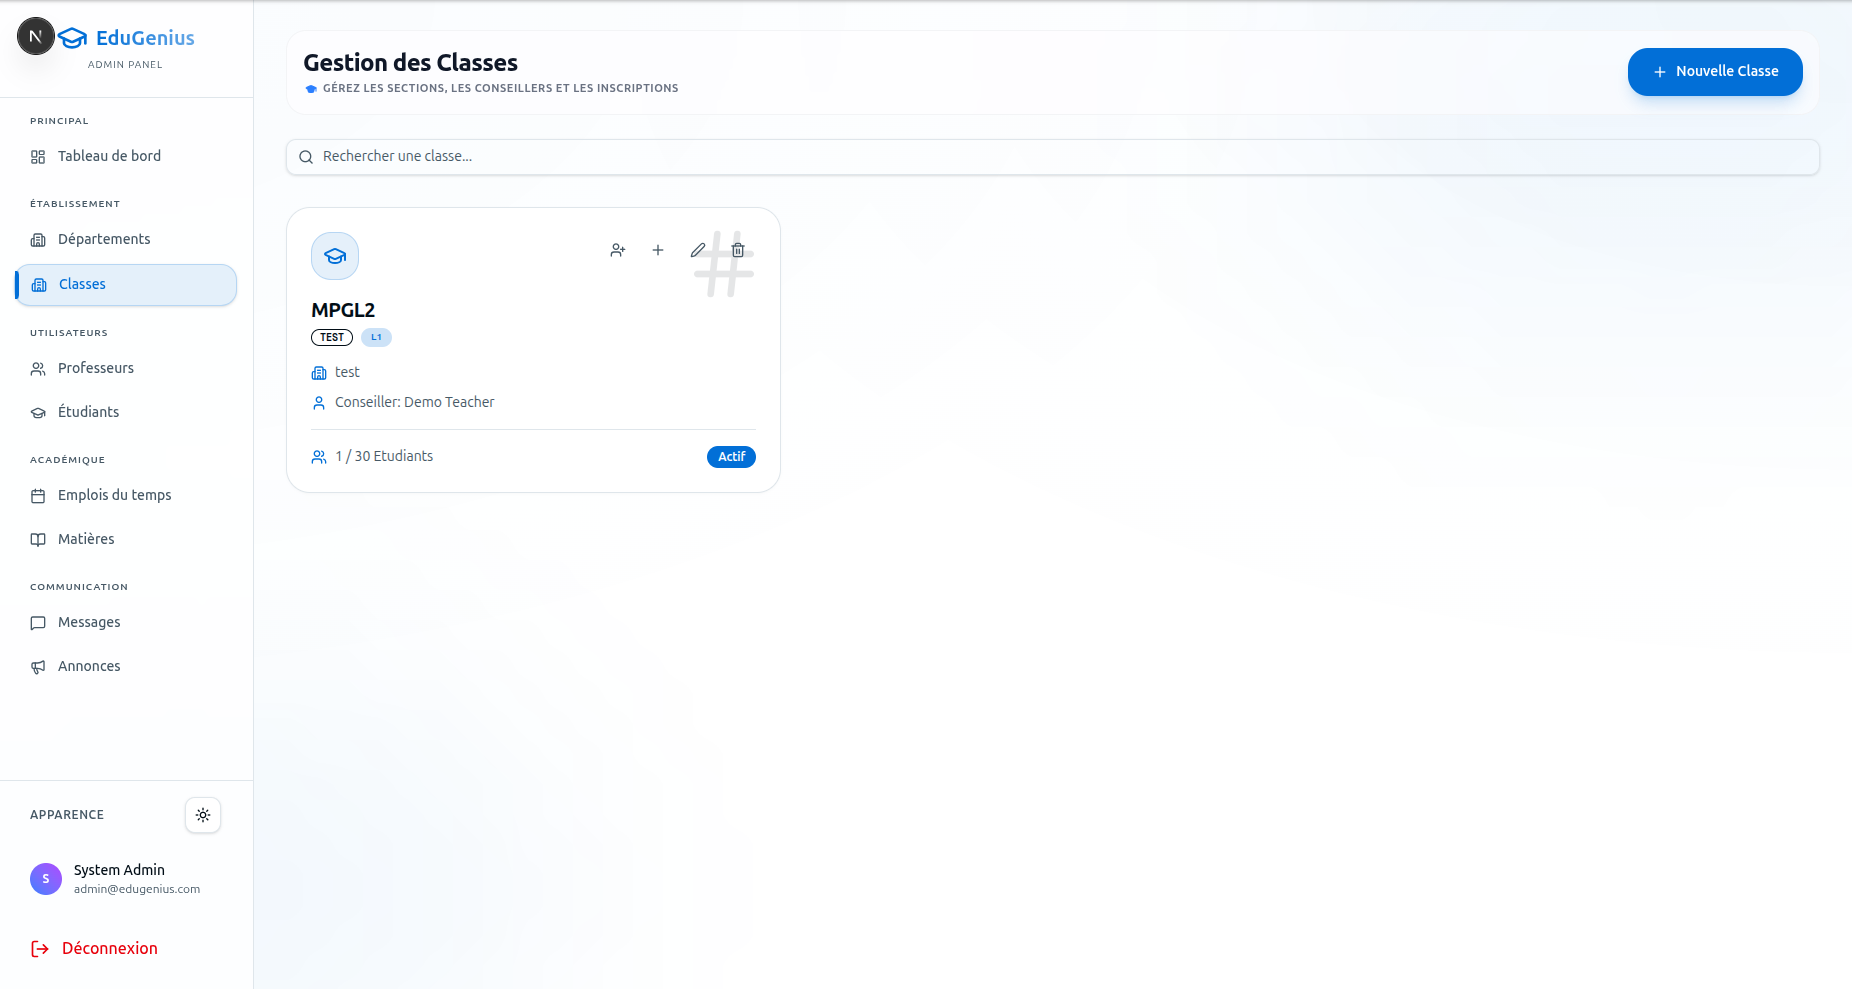
\includegraphics[width=\textwidth]{images/class_management_ui_1.png}
    \caption{Interface de gestion des classes : Liste générale}
    \label{fig:class_list_ui}
\end{figure}

\begin{figure}[H]
    \centering
    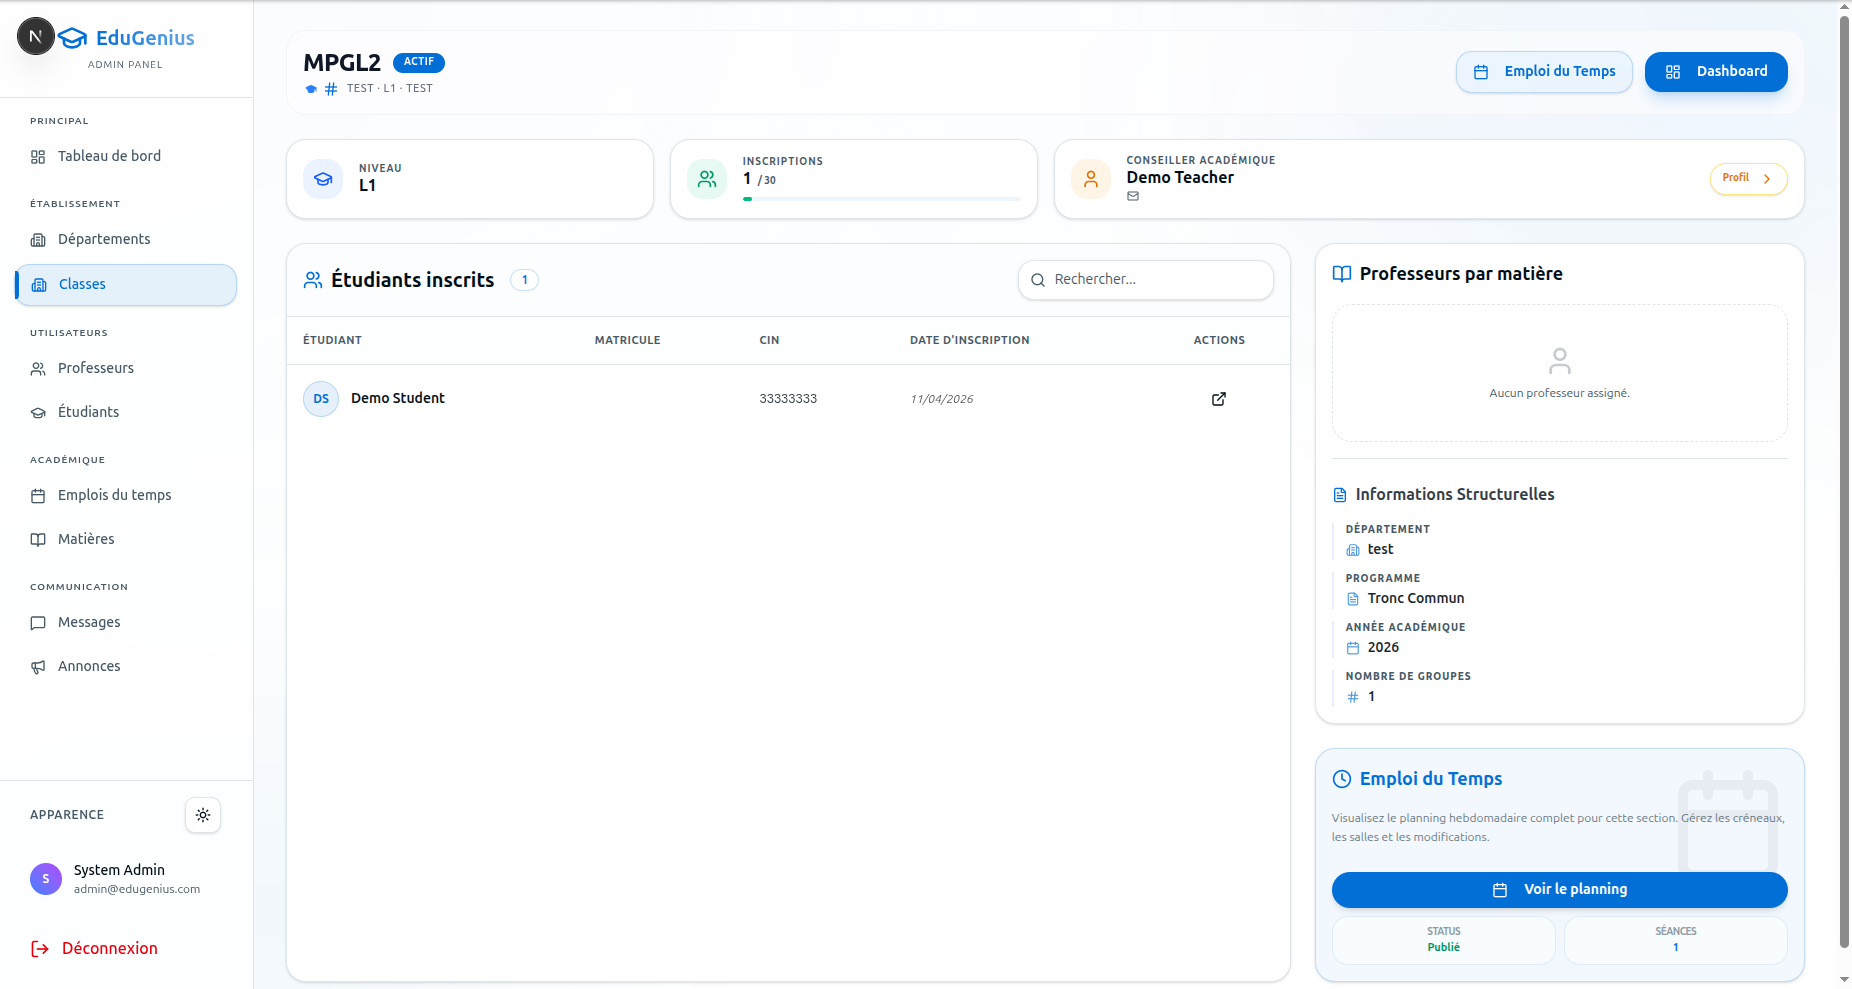
\includegraphics[width=\textwidth]{images/class_management_ui_2.png}
    \caption{Interface de création et d'édition des classes}
    \label{fig:class_form_ui}
\end{figure}

\subsection{Interface de planification des cours}

La création d'un emploi du temps suit un assistant en trois étapes : (1) informations générales (titre, année, semestre, classe/enseignant cible), (2) configuration des séances avec détection de conflits d'horaires et support de la récurrence, (3) récapitulatif avec validation et publication.

\begin{figure}[H]
    \centering
    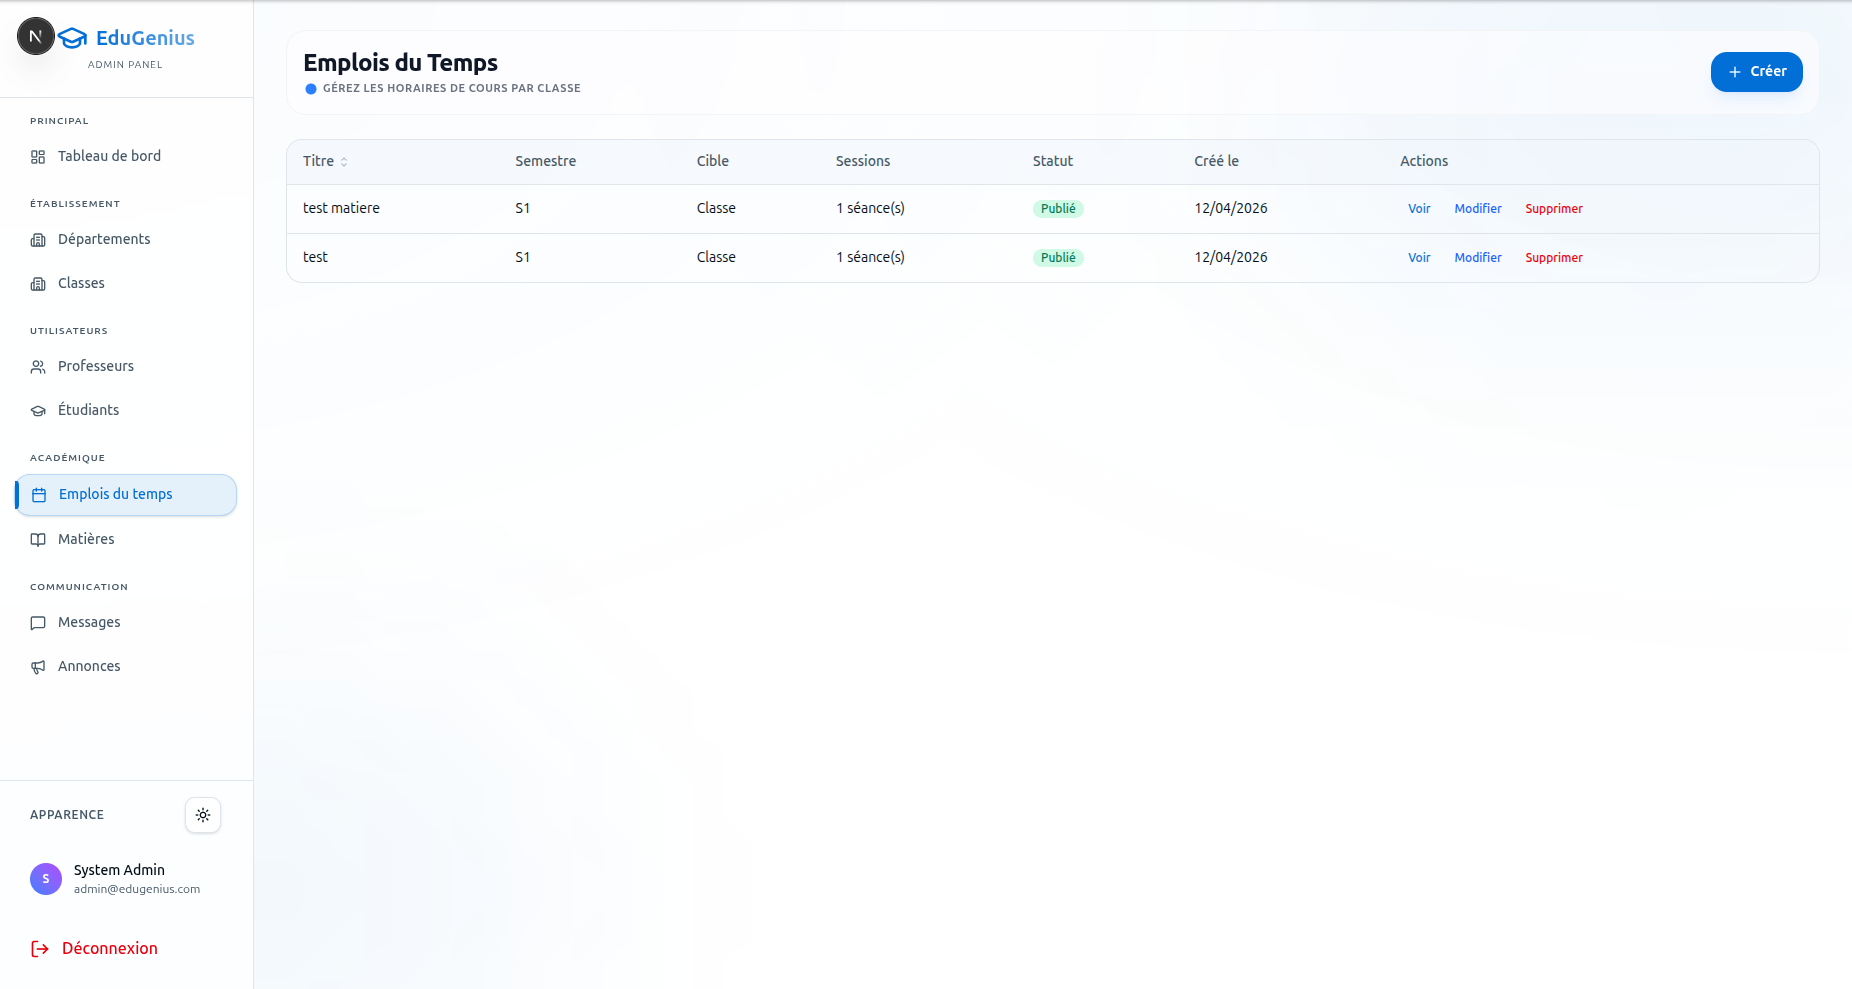
\includegraphics[width=\textwidth]{images/schedule_management_ui_1.png}
    \caption{Interface de planification : Informations générales}
    \label{fig:schedule_ui_1}
\end{figure}

\begin{figure}[H]
    \centering
    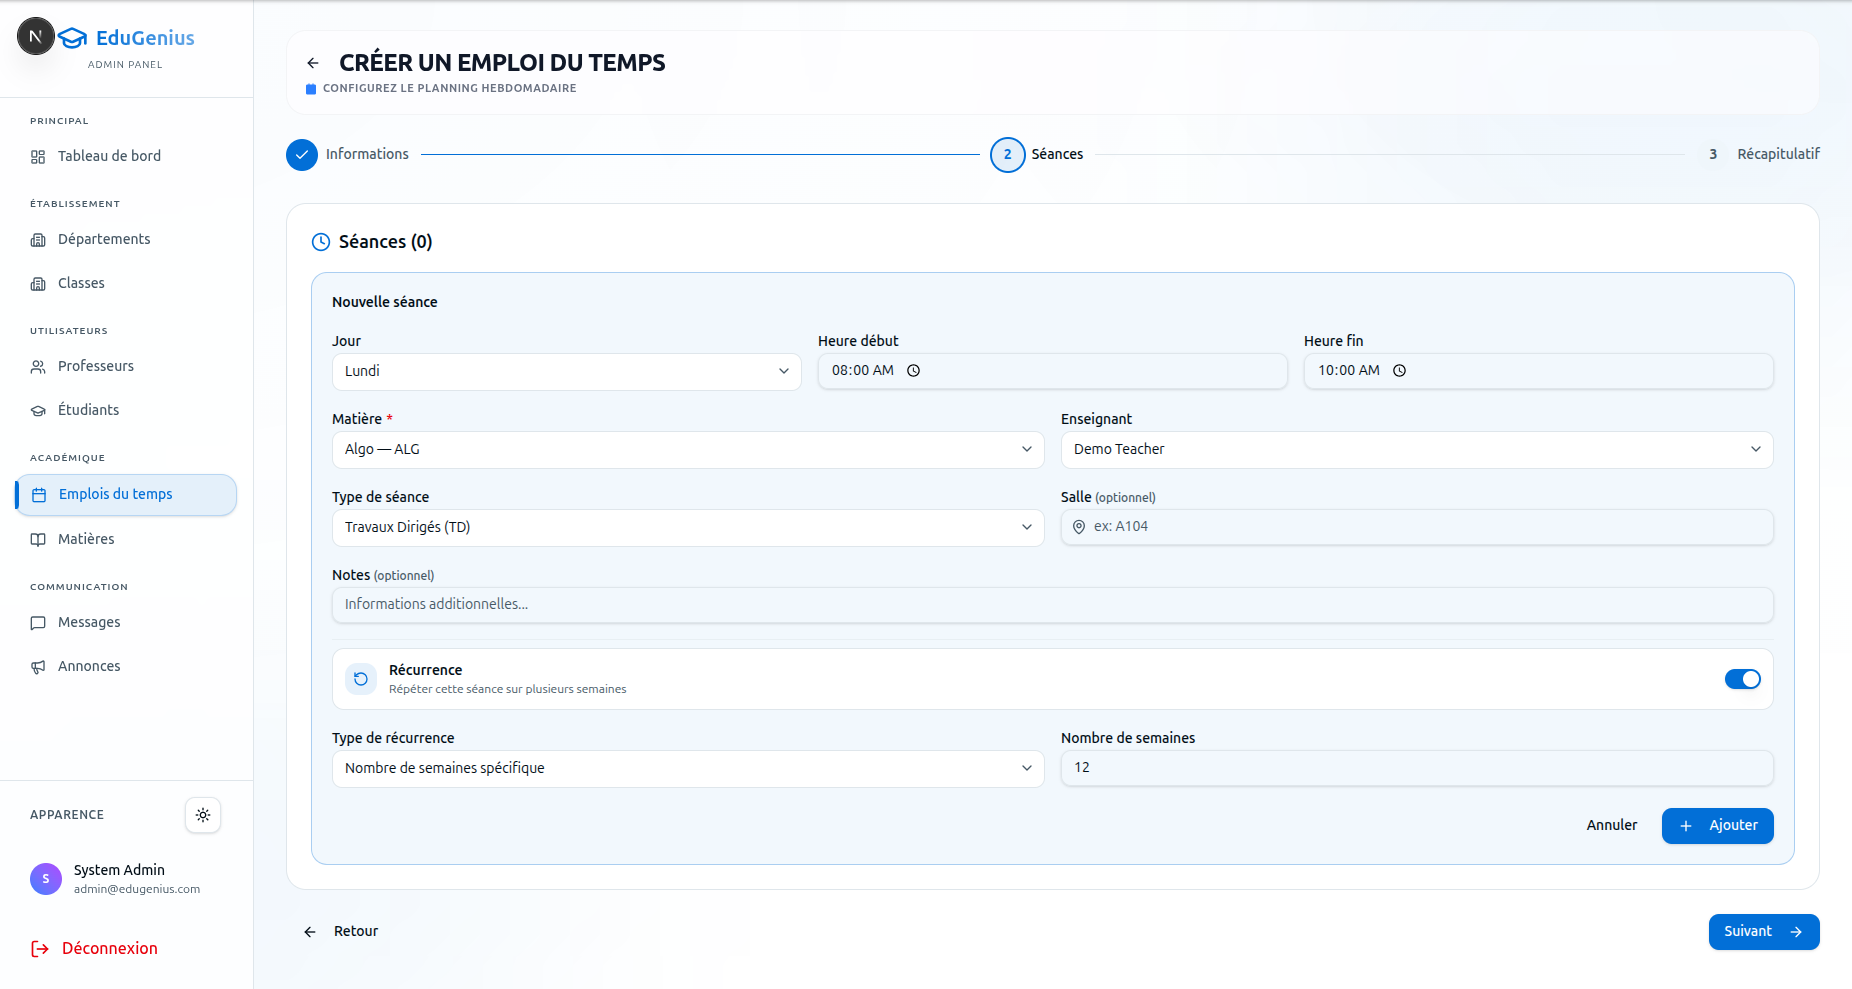
\includegraphics[width=\textwidth]{images/schedule_management_ui_2.png}
    \caption{Interface de planification : Configuration des séances}
    \label{fig:schedule_ui_2}
\end{figure}

\begin{figure}[H]
    \centering
    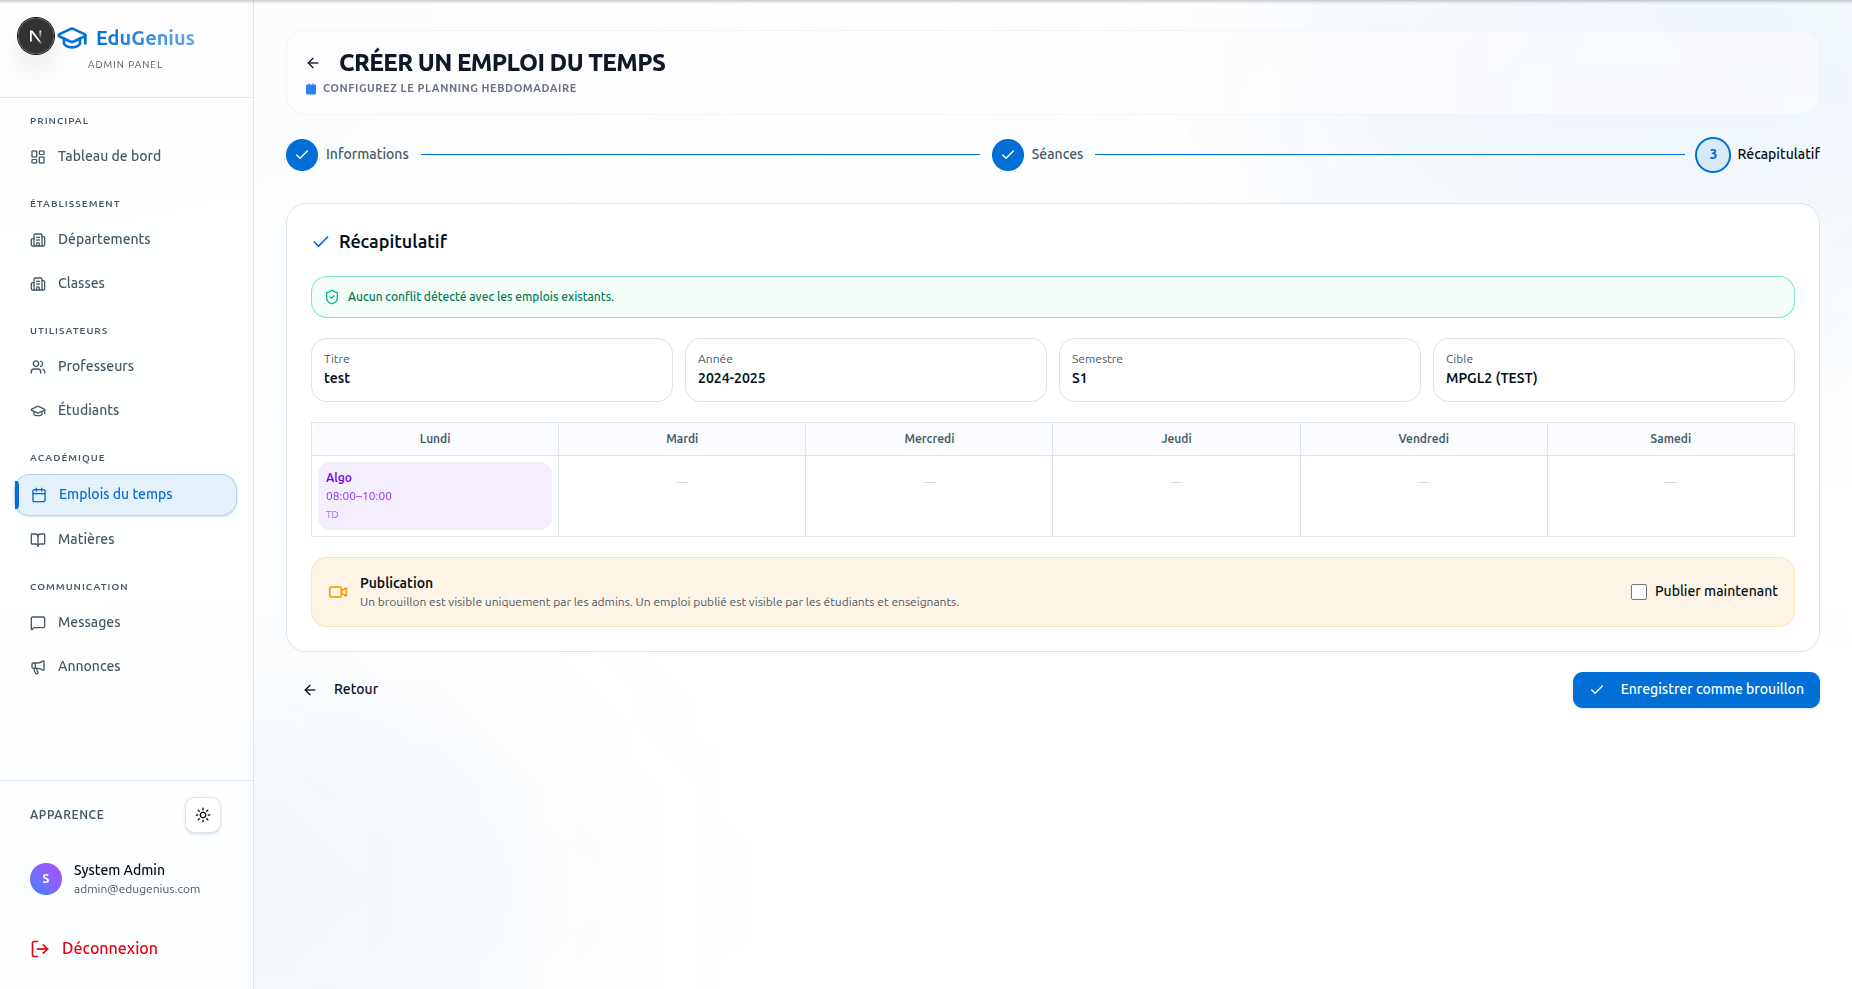
\includegraphics[width=\textwidth]{images/schedule_management_ui_3.png}
    \caption{Interface de planification : Récapitulatif et validation}
    \label{fig:schedule_ui_3}
\end{figure}

\subsection{Interface de supervision générale (Admin)}

Le tableau de bord de supervision offre un aperçu global de la plateforme : indicateurs clés (effectifs, classes, sessions en direct, taux de présence), sessions actives avec possibilité de rejoindre, dernières annonces et travaux soumis, distribution des effectifs par classe, et alertes système.

\begin{figure}[H]
    \centering
    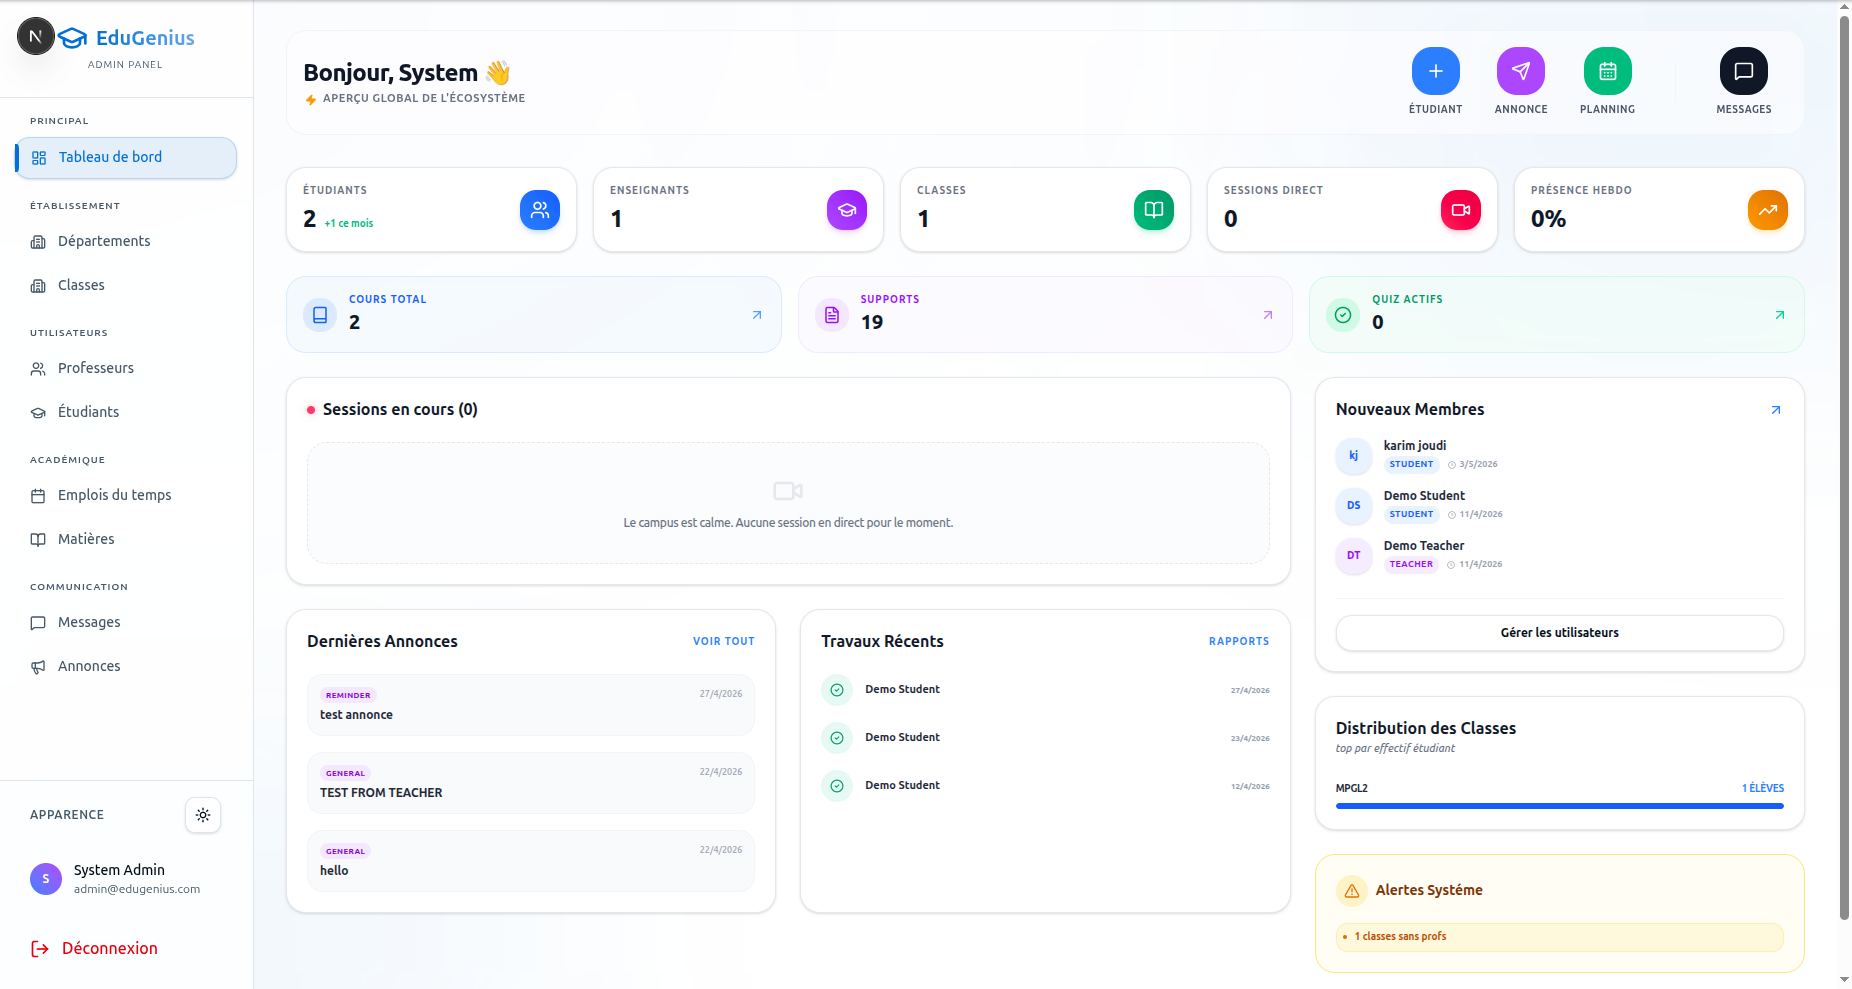
\includegraphics[width=\textwidth]{images/supervision_admin_ui.png}
    \caption{Tableau de bord de supervision}
    \label{fig:supervision_ui}
\end{figure}
\subsection{Interface de suivi de présence et historique}

L'historique de présence permet de filtrer par période et d'afficher les statistiques consolidées (taux de présence moyen, nombre de présents, retardataires et absents). Un tableau détaillé présente chaque session avec son taux d'assiduité, et un export CSV est disponible.

\begin{figure}[H]
    \centering
    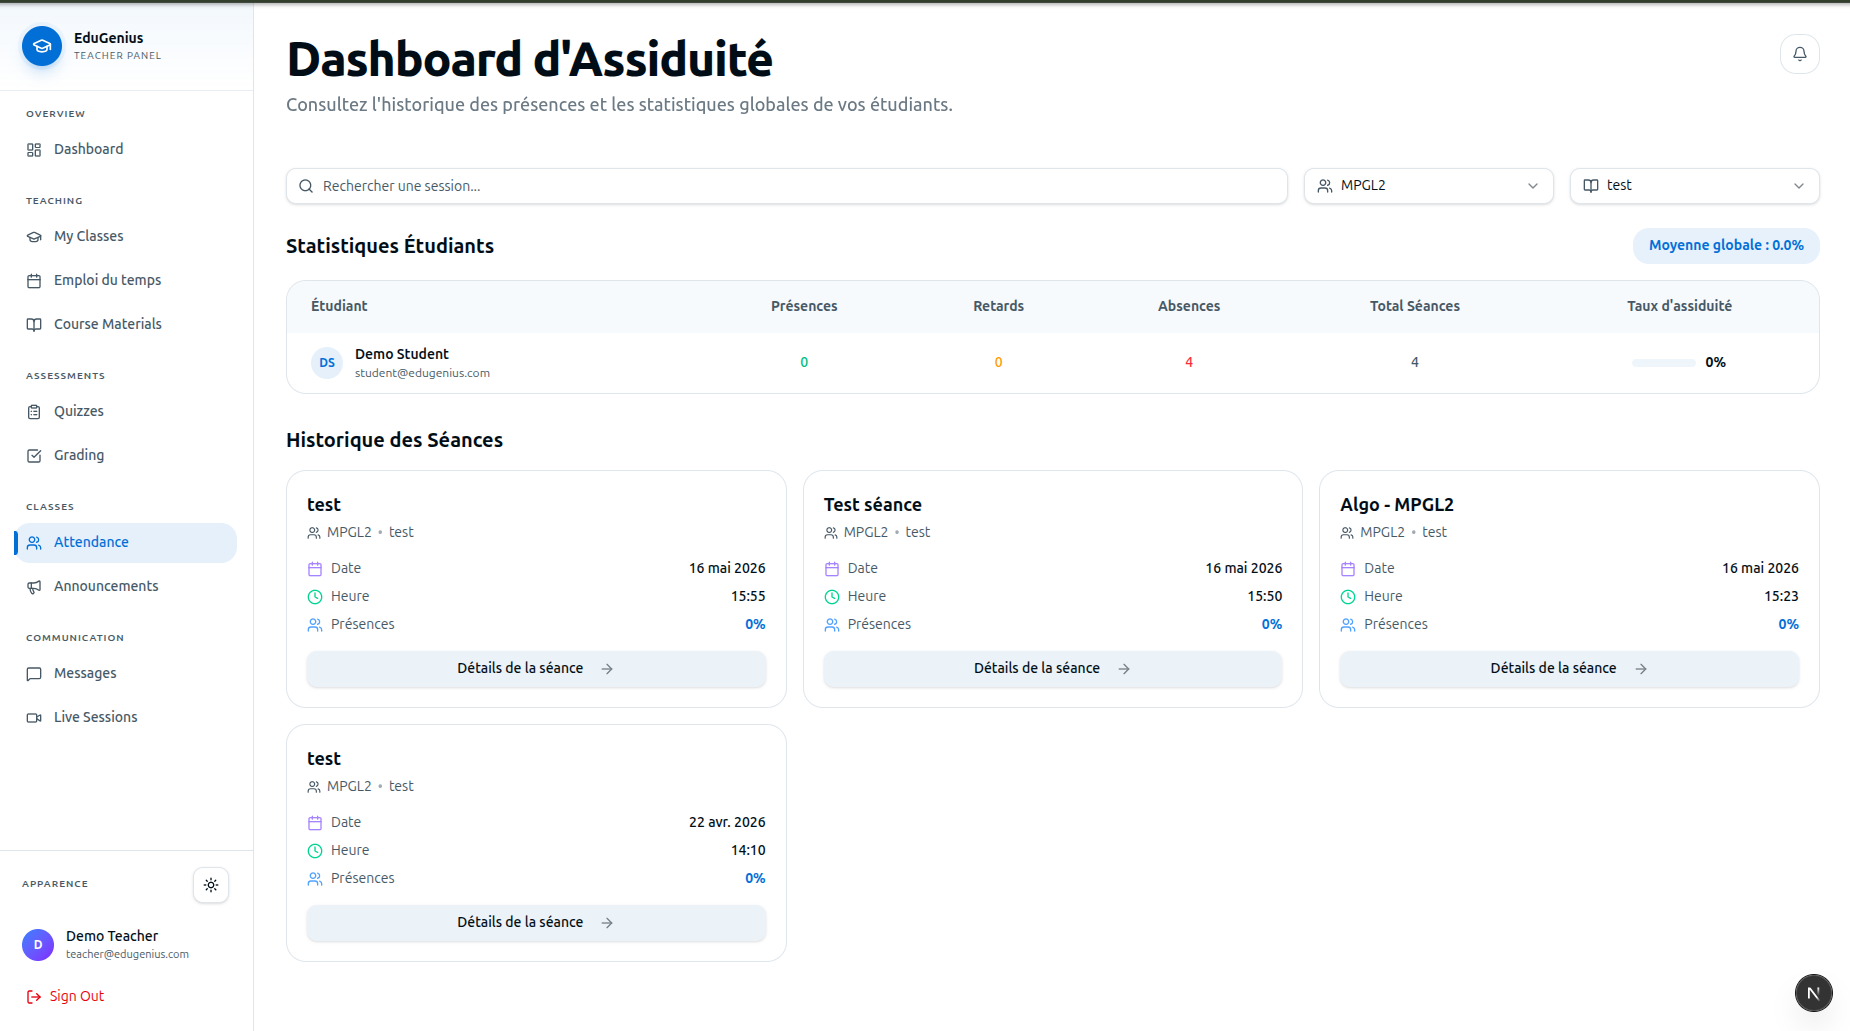
\includegraphics[width=\textwidth]{images/presence_ui.png}
    \caption{Historique des participations par étudiant/session}
    \label{fig:presence_ui}
\end{figure}

\subsection{Interface de replay (enregistrement)}

Les sessions enregistrées sont accessibles via un onglet dédié dans l'espace étudiant. Chaque enregistrement est présenté sous forme de carte avec le nom de la classe, le titre de la session, l'enseignant et la durée. L'interface propose également un onglet pour les sessions à venir avec indication du statut (planifié/en direct).

\begin{figure}[H]
    \centering
    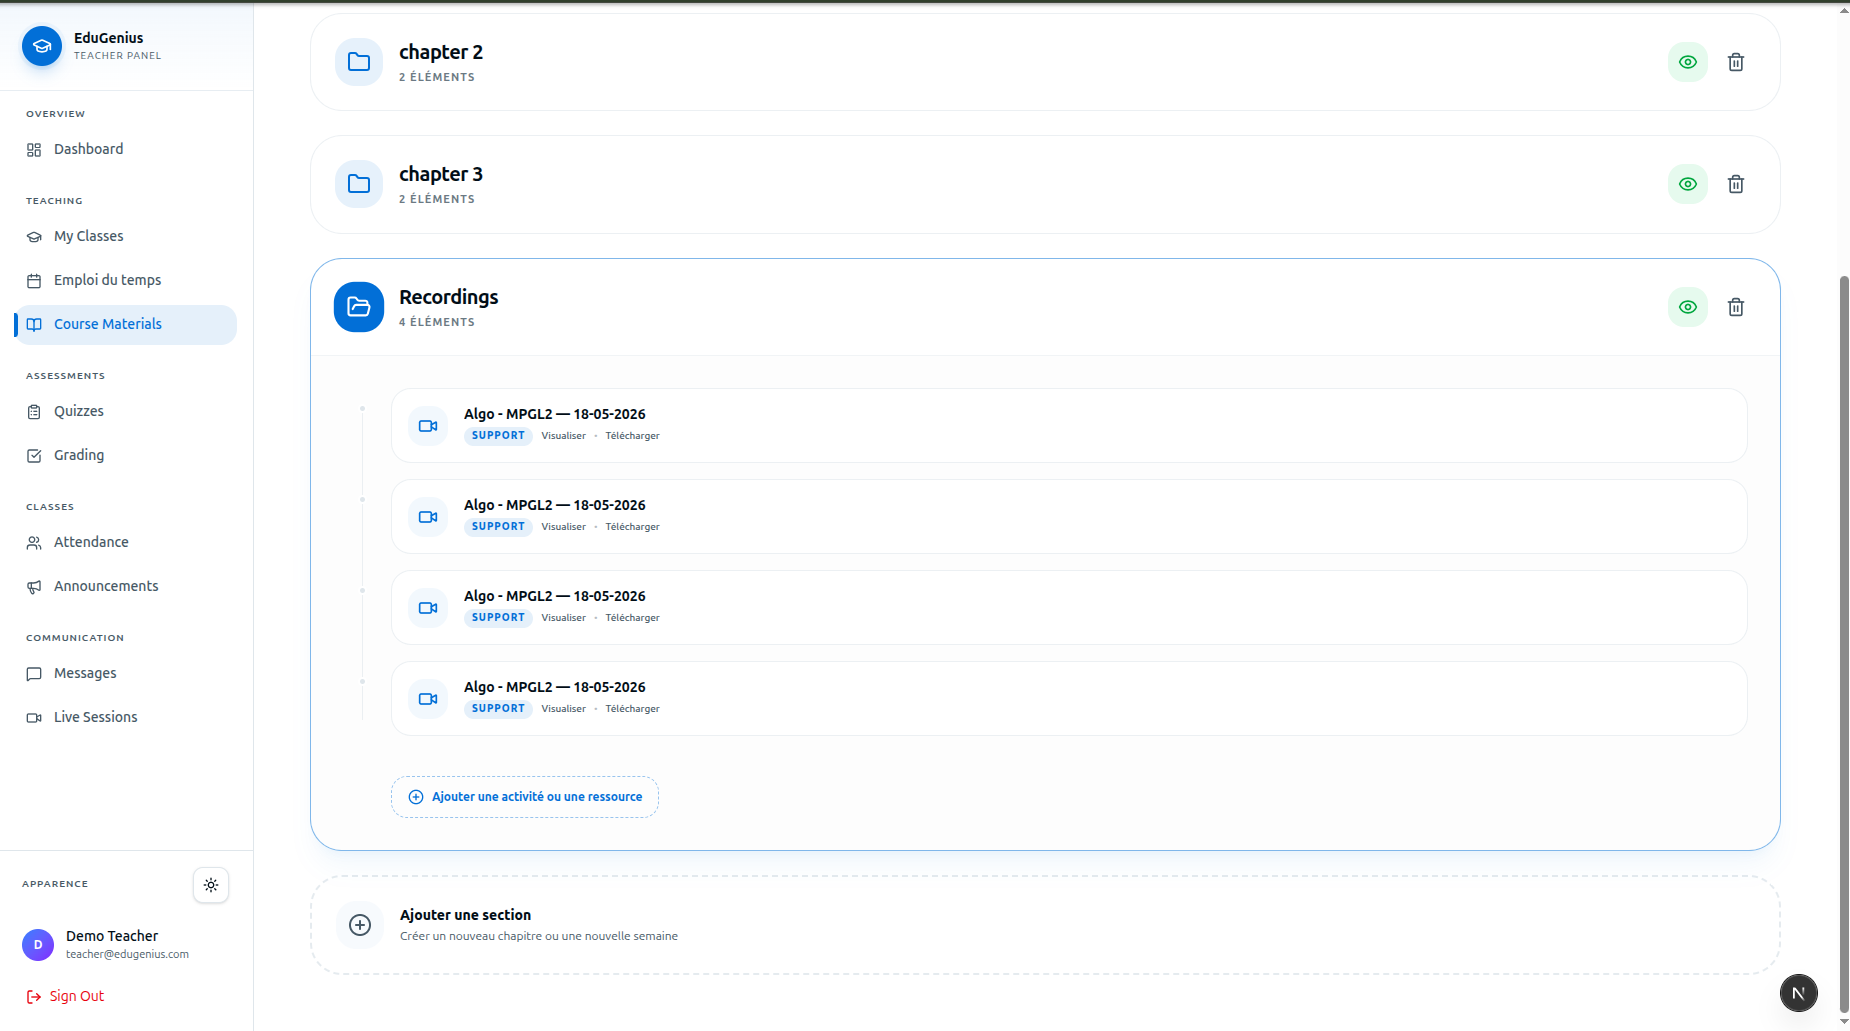
\includegraphics[width=\textwidth]{images/replay_ui_1.png}
    \caption{Interface de replay : Dossier des enregistrements disponibles par classe et matière}
    \label{fig:replay_list_ui}
\end{figure}

\section{Tests}
Cette phase de tests garantit la fiabilité des algorithmes de détection de présence et la robustesse de la gestion administrative des classes.

\subsection{Tests unitaires}
Nous avons mis en place des tests automatisés avec \textbf{Jest} pour valider la logique métier de calcul d'assiduité. La fonction \texttt{calculateAttendance} a été extraite et testée de manière isolée avec deux scénarios critiques :
\begin{itemize}
    \item \textbf{Validation des seuils} : Un étudiant participant à 30 minutes sur 60 (50\%) est marqué "Absent" car son taux est inférieur au seuil de 70\% (\texttt{attendanceThreshold}).
    \item \textbf{Détection des retards} : Un étudiant rejoignant la session à 09h20 pour un cours débutant à 09h00 est marqué "Late" car il dépasse la \texttt{gracePeriod} de 15 minutes.
\end{itemize}

\begin{figure}[H]
    \centering
    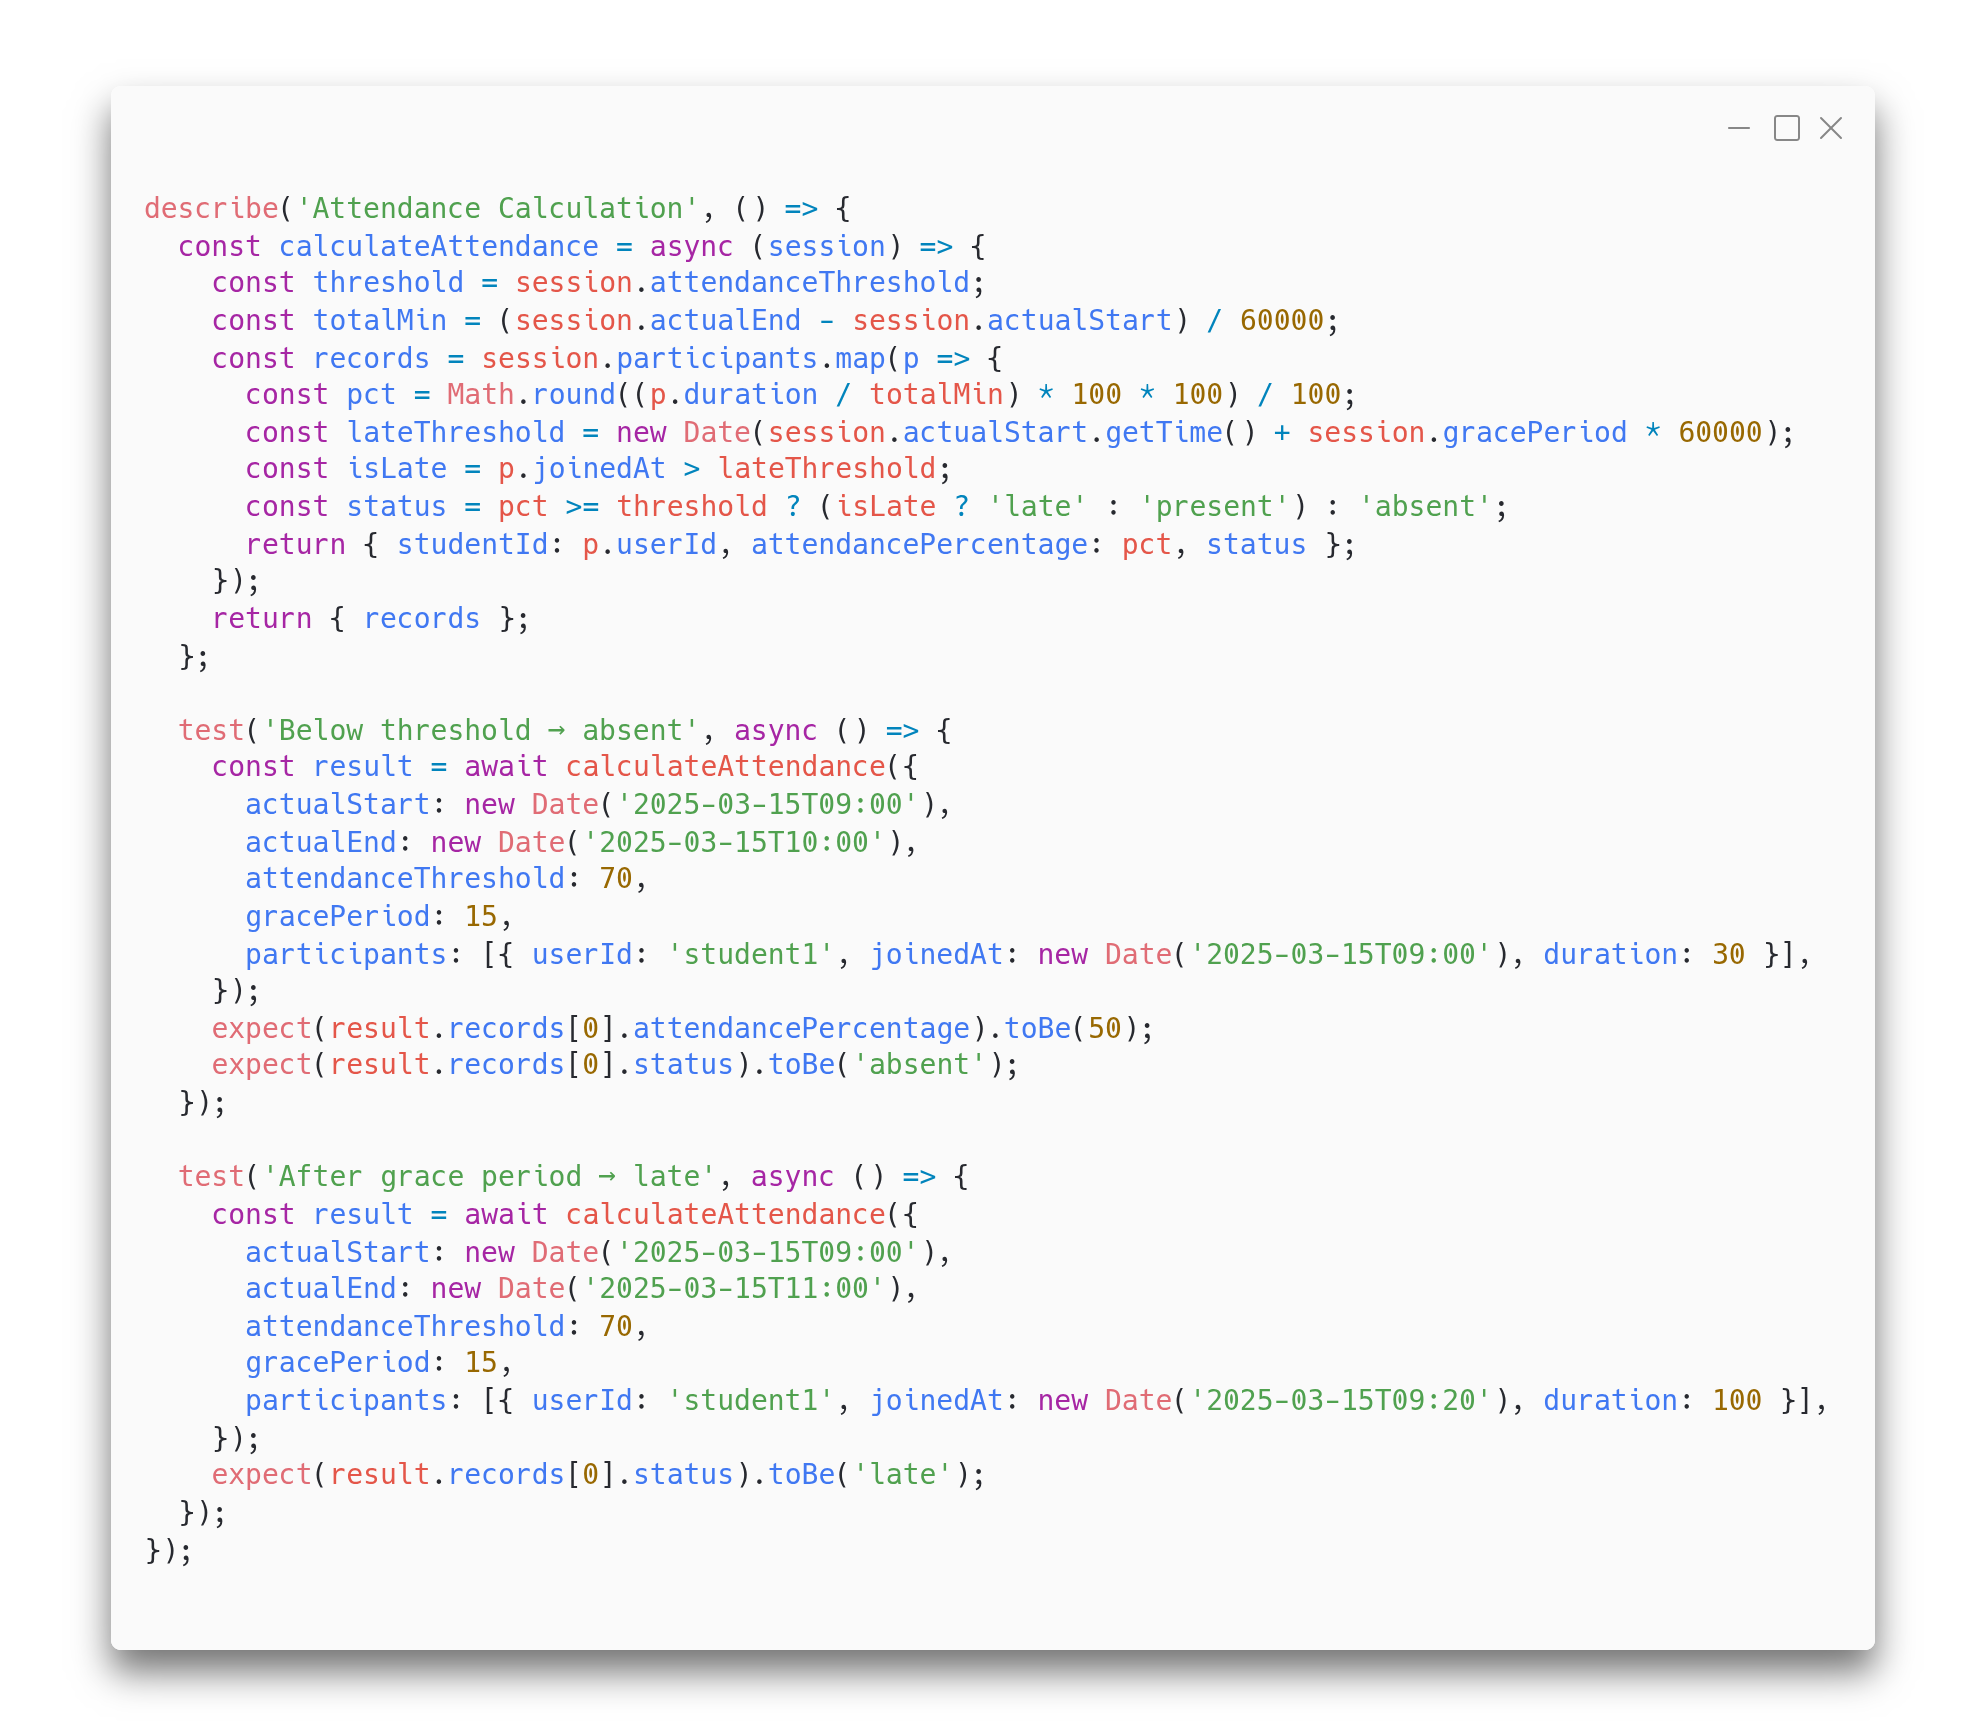
\includegraphics[width=0.9\textwidth]{images/attence_test.png}
    \caption{Extrait du code source du test unitaire (Jest)}
    \label{fig:unit_test_code_s2}
\end{figure}

\subsection{Tests d’intégration}
Les tests d'intégration valident la communication entre le client HTTP, le serveur Express et la base de données MongoDB. Le test principal a porté sur la création d'un emploi du temps via l'endpoint \texttt{POST /api/admin/schedules}.

À l'aide de l'outil \textbf{Postman}, nous avons soumis une requête authentifiée avec le token JWT d'un administrateur, contenant les informations de l'emploi du temps (titre, année universitaire, semestre, classe cible, séances). Le système a validé avec succès la chaîne complète : extraction du token $\rightarrow$ vérification des droits d'administrateur $\rightarrow$ validation et persistance dans MongoDB $\rightarrow$ génération automatique des URLs de visioconférence $\rightarrow$ retour de l'objet créé.

Comme illustré dans la figure \ref{fig:integration_test_s2}, le serveur retourne un statut \texttt{201 Created} accompagné de l'objet JSON de l'emploi du temps. La réponse inclut l'identifiant unique généré par MongoDB (\texttt{\_id}), les séances planifiées avec leurs créneaux horaires, ainsi que l'URL de visioconférence Jitsi automatiquement générée (\texttt{meetingUrl}). Ce test confirme le bon fonctionnement du module de planification, brique centrale de l'organisation pédagogique du sprint.

\begin{figure}[H]
    \centering
    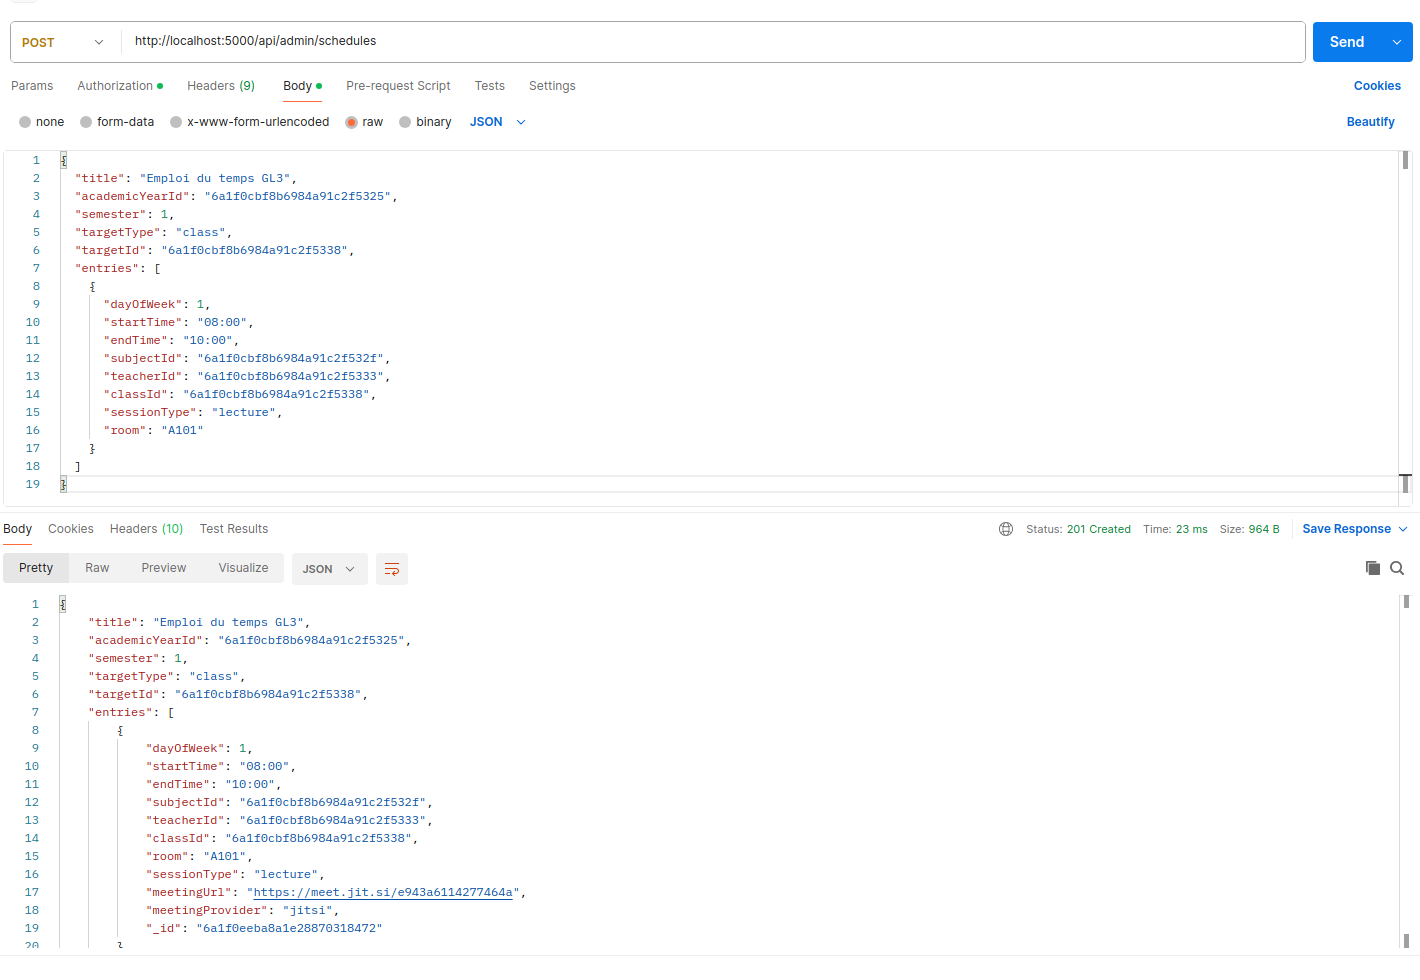
\includegraphics[width=0.8\textwidth]{images/integration_test_sprint_2.png}
    \caption{Validation du point d'entrée POST /api/admin/schedules via Postman}
    \label{fig:integration_test_s2}
\end{figure}

\subsection{Tests fonctionnels}
Les tests de bout en bout ont validé le parcours utilisateur complet de création et configuration d'une classe :
\begin{enumerate}
    \item L'administrateur accède à la page \texttt{/admin/classes} et clique sur \textbf{Nouvelle Classe}.
    \item Il remplit le formulaire (nom, code, département, niveau, capacité) et soumet.
    \item La classe apparaît dans la grille avec son code et son niveau.
    \item L'administrateur inscrit des étudiants via la modale d'inscription avec recherche.
\end{enumerate}

\begin{figure}[H]
    \centering
    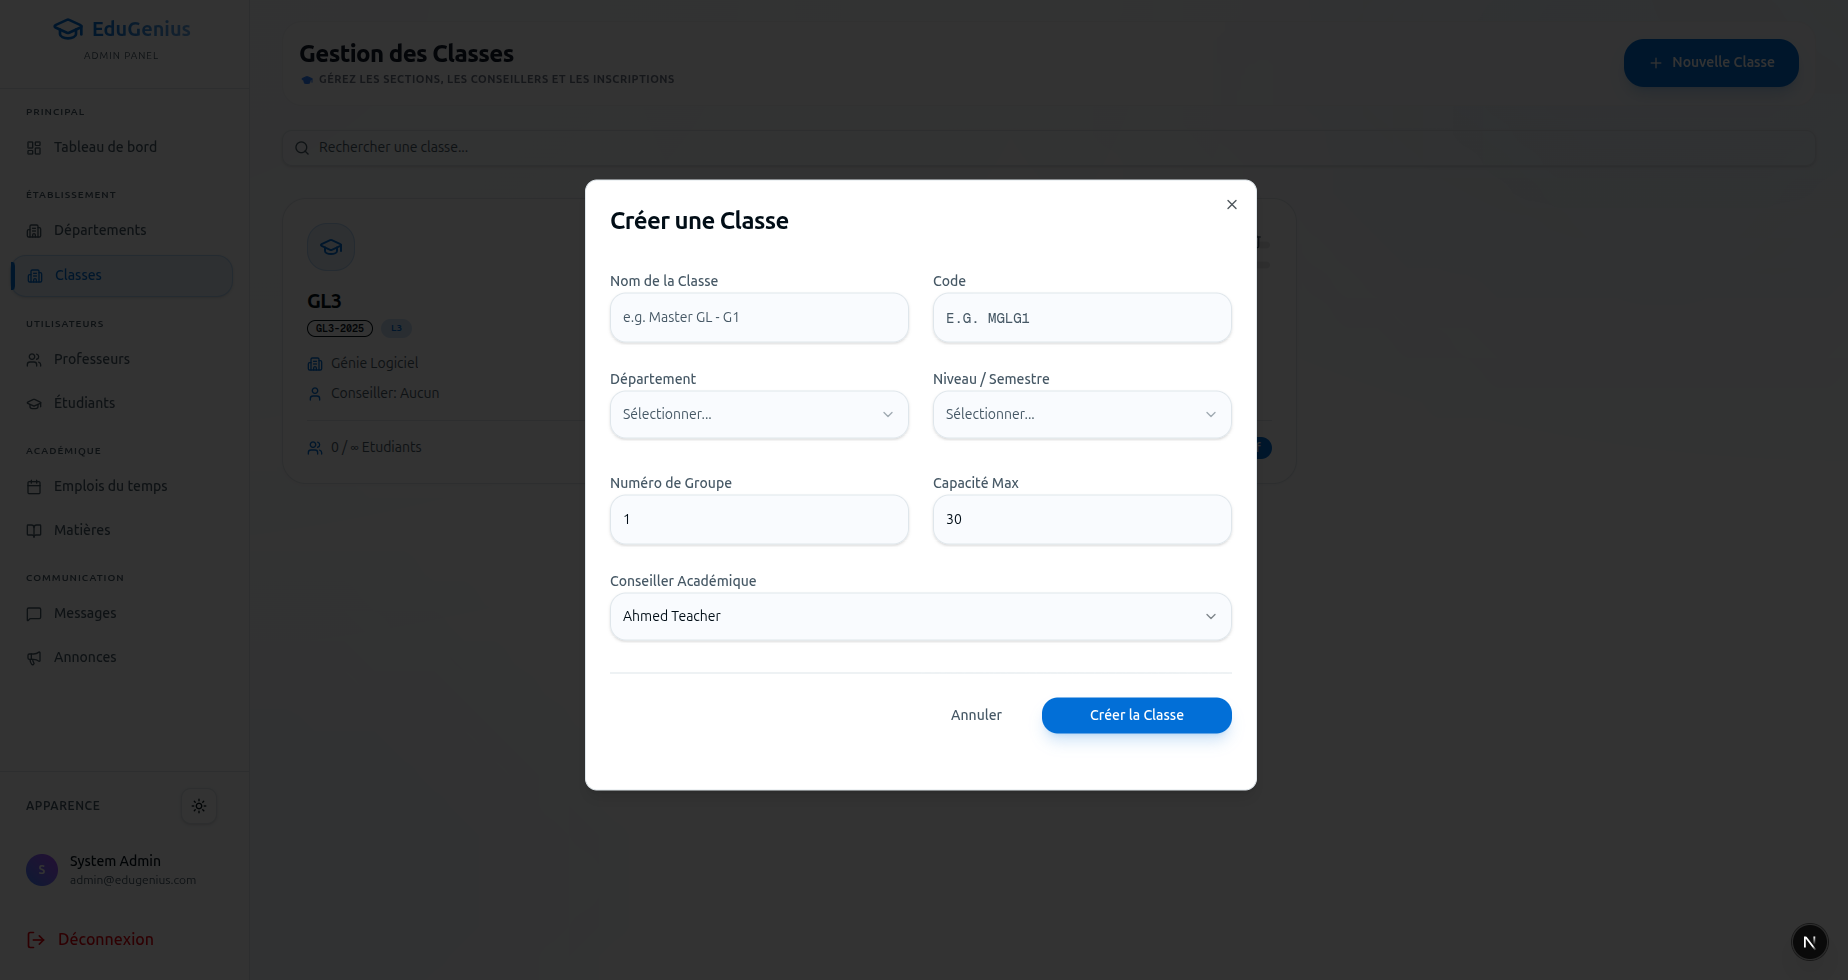
\includegraphics[width=0.9\textwidth]{images/functional_test_sprint_2.png}
    \caption{Parcours fonctionnel de création et configuration d'une classe}
    \label{fig:functional_test_s2}
\end{figure}

\section{Conclusion}

Ce deuxième sprint a permis de doter EduGenius d’un socle complet de gestion des classes, de planification et de visioconférence. L’ensemble des onze user stories (US-06 à US-16) a été développé et testé avec succès, offrant une base solide pour les fonctionnalités pédagogiques du sprint 3.
